\documentclass[12pt, a4paper]{article}

% --- Pacotes Fundamentais ---
\usepackage[utf8]{inputenc}
\usepackage[T1]{fontenc}
\usepackage[brazilian]{babel}
\usepackage{amsmath, amssymb}
\usepackage{graphicx}
\usepackage{booktabs}
\usepackage{array}
\usepackage{caption}
\usepackage{subcaption}
\usepackage{hyperref}
\usepackage{geometry}
\usepackage{float}

% Caminhos de busca para gráficos e figuras
\graphicspath{{../../graficos/metaheuristicas/}{graficos/metaheuristicas/}{../../graficos/}{graficos/}}

\geometry{margin=2.5cm}

\title{\textbf{Avaliação Experimental de Metaheurísticas e Busca Local no Problema do Caixeiro Viajante: Análise Comparativa com Heurísticas Construtivas de Referência}}
\author{Bernardo Vale dos Santos Bento}
\date{Outubro de 2026}

\begin{document}

\maketitle

\begin{abstract}
Este trabalho expande a avaliação experimental de métodos de resolução aproximada para o Problema do Caixeiro Viajante (\textit{Traveling Salesman Problem} --- TSP), avaliando o comportamento e o custo computacional de técnicas de busca local e metaheurísticas estocásticas em contraste com heurísticas construtivas de referência. Foram implementadas e comparadas a Busca Local 2-Opt clássica acelerada por \textit{Don't-Look Bits} com cálculo de ganho em $\mathcal{O}(1)$ e a metaheurística \textit{Simulated Annealing} (SA) com resfriamento geométrico e vizinhança 2-opt. Avaliaram-se empiricamente duas estratégias de inicialização: Partida Aleatória (\textit{Random Start}) e Partida Informada (\textit{Warm Start / Low-Temperature Start}) a partir de rota construtiva de alta qualidade. O desempenho das metaheurísticas foi medido em 21 instâncias \textit{benchmark} da TSPLIB e comparado diretamente com as duas melhores heurísticas construtivas da etapa anterior deste projeto: \textit{Farthest Insertion} (H5) e \textit{Centroid-Based Insertion} (H1). Os resultados mostram que a busca local 2-opt isolada a partir de rotas aleatórias fica presa precocemente em mínimos locais de baixa qualidade (custo relativo médio de $1{,}261\times$). Em contrapartida, quando empregada como pós-otimizador local sobre rota de \textit{warm start}, o 2-opt atinge $1{,}026\times$ em apenas $7{,}71\,\mathrm{ms}$. No topo da acurácia global, o \textit{Simulated Annealing} com partida aleatória atinge a maior qualidade média do estudo ($1{,}005\times$) com tempo médio de $1{,}74\,\mathrm{s}$, enquanto o SA com \textit{Low-Temperature Start} converge $4{,}2$ vezes mais rápido ($411{,}84\,\mathrm{ms}$) com perda residual mínima de qualidade ($1{,}015\times$).
\end{abstract}

% -------------------------------------------------------
\section{Contextualização e Abordagens Avaliadas}
% -------------------------------------------------------

Na fase preliminar deste projeto \cite{bento2026}, foram avaliadas seis heurísticas puramente construtivas sobre 21 instâncias padronizadas da biblioteca TSPLIB \cite{reinelt1991}: \textit{Nearest Neighbor} (H4) \cite{rosenkrantz1977}, \textit{Farthest Insertion} (H5) \cite{rosenkrantz1977}, \textit{Greedy Edge} (H6) \cite{bentley1992}, \textit{Centroid-Based Insertion} (H1), \textit{Eccentricity Insertion} (H2) e \textit{Hybrid-Score Insertion} (H3).

Daquele processo experimental, destacaram-se como as duas melhores heurísticas:
\begin{enumerate}
    \item \textbf{H5 (\textit{Farthest Insertion})}: melhor qualidade média de solução entre as abordagens construtivas puras, com custo médio de $35.429$ e tempo computacional de $5{,}99\,\mathrm{ms}$.
    \item \textbf{H1 (\textit{Centroid-Based Insertion})}: melhor equilíbrio de tempo e qualidade na Fronteira de Pareto das construtivas, operando com custo médio de $36.292$ e tempo de apenas $3{,}33\,\mathrm{ms}$.
\end{enumerate}

Nesta nova etapa, a avaliação experimental é expandida para metaheurísticas e busca local, fundamentando-se nos estudos de Johnson e McGeoch \cite{johnson1997}. Foram implementadas duas metodologias:
\begin{itemize}
    \item \textbf{Busca Local 2-Opt Clássica} \cite{croes1958, lin1965}: algoritmo de descida estrita com poda de arestas via \textit{Don't-Look Bits} \cite{bentley1992} e avaliação analítica da variação de custo em tempo constante $\mathcal{O}(1)$.
    \item \textbf{Simulated Annealing (SA)} \cite{kirkpatrick1983, cerny1985}: metaheurística baseada no recozimento físico metalúrgico, que aceita estocasticamente movimentos de piora sob o critério de Metropolis para escapar de mínimos locais.
\end{itemize}

Ambas as abordagens foram avaliadas sob duas estratégias de partida:
\begin{itemize}
    \item \textbf{Partida Aleatória (\textit{Random Start})}: inicialização a partir de uma permutação aleatória dos vértices, sem informação geométrica inicial.
    \item \textbf{Partida Informada (\textit{Warm Start / Low-Temperature Start})}: inicialização a partir da melhor rota gerada no ciclo anterior (H5 --- \textit{Farthest Insertion}), explorando o refinamento local de arestas.
\end{itemize}

% -------------------------------------------------------
\section{Modelagem Matemática e Métricas de Avaliação}
% -------------------------------------------------------

\subsection{Formulações de Distâncias na TSPLIB}

Considera-se um grafo completo não direcionado $G = (V, E)$, onde $V = \{1, 2, \dots, n\}$ representa o conjunto de $n$ vértices com coordenadas bidimensionais $(x_i, y_i) \in \mathbb{R}^2$, e $E$ representa o conjunto de arestas ponderadas por uma função de custo $d: V \times V \to \mathbb{R}^+$. A rota é representada como uma permutação cíclica $\pi = (\pi_1, \pi_2, \dots, \pi_n)$, cujo custo total é dado por:
\begin{equation}
    C(\pi) = d(\pi_n, \pi_1) + \sum_{i=1}^{n-1} d(\pi_i, \pi_{i+1})
\end{equation}

O cômputo das distâncias segue estritamente as especificações oficiais da TSPLIB \cite{reinelt1991}:
\begin{enumerate}
    \item \textbf{Distância Pseudo-Euclidiana (\texttt{ATT})}: aplicada à instância \texttt{att48.tsp}. Dados $\Delta x = x_i - x_j$ e $\Delta y = y_i - y_j$, obtém-se o raio $r_{ij} = \sqrt{(\Delta x^2 + \Delta y^2)/10{,}0}$, o valor aproximado $t_{ij} = \mathrm{nint}(r_{ij})$ com $\mathrm{nint}(z) = \lfloor z + 0{,}5 \rfloor$, e a distância:
          \begin{equation}
              d_{ij} = \begin{cases} t_{ij} + 1, & \text{se } t_{ij} < r_{ij} \\ t_{ij}, & \text{caso contrário} \end{cases}
          \end{equation}
    \item \textbf{Distância Euclidiana Bidimensional (\texttt{EUC\_2D})}: aplicada às demais 20 instâncias:
          \begin{equation}
              d_{ij} = \mathrm{nint}\left(\sqrt{(x_i - x_j)^2 + (y_i - y_j)^2}\right)
          \end{equation}
\end{enumerate}

\subsection{Métricas de Avaliação de Desempenho}

Para comparar o desempenho de forma homogênea entre instâncias com dimensões variando de 48 a 200 vértices, definem-se as seguintes métricas sobre o conjunto de testes $\mathcal{I} = \{\mathcal{I}_1, \dots, \mathcal{I}_{21}\}$:

\paragraph{Custo Médio Absoluto.} Média aritmética dos custos obtidos pelo método $m$ nas 21 instâncias:
\begin{equation}
    \overline{C}(m) = \frac{1}{21} \sum_{i=1}^{21} C(m, \mathcal{I}_i)
\end{equation}

\paragraph{Custo Relativo e Custo Médio Relativo.} Para cada instância $\mathcal{I}_i$, o Custo Relativo de um método $m$ é normalizado pela melhor solução encontrada entre todas as alternativas avaliadas naquela instância:
\begin{equation}
    \mathrm{CR}(m, \mathcal{I}_i) = \frac{C(m, \mathcal{I}_i)}{\displaystyle\min_{m' \in \mathcal{M}} C(m', \mathcal{I}_i)}
\end{equation}
onde $\mathcal{M}$ reúne as metaheurísticas e as duas heurísticas de referência. O Custo Médio Relativo sintetiza o indicador:
\begin{equation}
    \overline{\mathrm{CR}}(m) = \frac{1}{21} \sum_{i=1}^{21} \mathrm{CR}(m, \mathcal{I}_i)
\end{equation}

\paragraph{Tempo Computacional Médio.} Tempo de execução em milissegundos ($ms$) medido via \texttt{time.perf\_counter()}, agregado pela média aritmética $\overline{T}(m)$.

% -------------------------------------------------------
\section{Fundamentos e Modelagem das Metaheurísticas e Busca Local}
% -------------------------------------------------------

\subsection{O Operador 2-Opt e Avaliação em Tempo Constante \texorpdfstring{$\mathcal{O}(1)$}{O(1)}}

O movimento de troca 2-opt \cite{croes1958, lin1965} consiste na remoção de duas arestas não adjacentes $(u_1, u_2)$ e $(v_1, v_2)$ do circuito e sua reconexão invertendo a orientação do subcaminho intermediário entre $u_2$ e $v_1$:
\begin{align}
    \text{Circuito original:} &\quad (\dots, u_1) \to (u_2 \to \dots \to v_1) \to (v_2, \dots) \\
    \text{Após o movimento 2-opt:} &\quad (\dots, u_1) \to (v_1 \to \dots \to u_2) \to (v_2, \dots)
\end{align}

Em problemas geométricos euclidianos, o operador 2-opt desfaz cruzamentos de arestas no plano. Para conferir eficiência computacional, a variação de custo $\Delta$ é avaliada estritamente em tempo constante $\mathcal{O}(1)$:
\begin{equation}
    \Delta(u_1, u_2, v_1, v_2) = \left[ d(u_1, v_1) + d(u_2, v_2) \right] - \left[ d(u_1, u_2) + d(v_1, v_2) \right]
    \label{eq:delta_2opt}
\end{equation}
Um movimento é estritamente melhorante quando $\Delta < 0$, permitindo atualizar o custo do circuito de modo incremental através de $C_{\text{novo}} = C_{\text{atual}} + \Delta$.

\subsection{Busca Local 2-Opt Clássica Acelerada com Don't-Look Bits}

A busca local sistemática inspeciona pares de arestas em busca de melhorias. Para evitar que varreduras repetidas sobre nós estáveis degradem o tempo de execução, adota-se o mecanismo de \textit{Don't-Look Bits} \cite{bentley1992, johnson1997}:
\begin{enumerate}
    \item Cada vértice $i$ mantém uma flag booleana associada $\mathrm{dont\_look}[i]$, inicialmente desativada ($\mathrm{False}$).
    \item Se a flag de $i$ estiver ativada ($\mathrm{True}$), a inspeção de arestas incidentes a $i$ é ignorada na iteração.
    \item Caso a varredura completa da vizinhança de $i$ não produza nenhum movimento com $\Delta < 0$, ativa-se $\mathrm{dont\_look}[i] = \mathrm{True}$.
    \item Quando uma inversão bem-sucedida é executada entre as posições $i$ e $k$, reativam-se imediatamente os bits dos vértices envolvidos e de seus vizinhos na rota:
          \begin{equation}
              \mathrm{dont\_look}[i] = \mathrm{dont\_look}[k] = \mathrm{dont\_look}[i-1] = \mathrm{dont\_look}[k+1] = \mathrm{False}
          \end{equation}
    \item O algoritmo finaliza quando todos os bits tornam-se ativos, assegurando convergência a um \textbf{mínimo 2-ótimo estrito}.
\end{enumerate}

\subsection{Simulated Annealing (SA) Estocástico}

O \textit{Simulated Annealing} \cite{kirkpatrick1983, cerny1985} introduz um mecanismo estocástico de escape de mínimos locais:
\begin{itemize}
    \item A cada iteração sobre o circuito corrente com custo $C$, gera-se um circuito vizinho com perturbação 2-opt e variação $\Delta = C' - C$ calculada em $\mathcal{O}(1)$.
    \item Movimentos melhorantes ($\Delta \le 0$) são \textbf{sempre aceitos}.
    \item Movimentos degradantes ($\Delta > 0$) são aceitos com probabilidade de Metropolis:
          \begin{equation}
              P(\text{aceitar}) = \exp\left(-\frac{\Delta}{T}\right)
          \end{equation}
\end{itemize}

O resfriamento ocorre segundo um esquema geométrico $T_{k+1} = \alpha \cdot T_k$, com fator $\alpha \in [0{,}95, 0{,}98]$. Em cada patamar térmico, executam-se $L = \max(100, 5 \cdot n)$ tentativas. No caso da partida aleatória, a temperatura inicial $T_0$ é estimada por amostragem preliminar de movimentos com aumento de custo ($\overline{\Delta^+}$) para obter taxa inicial de aceitação de $80\%$, via $T_0 = -\overline{\Delta^+} / \ln(0{,}80)$. O processo cessa quando $T < T_{\mathrm{final}} = 10^{-3}$, preservando-se de forma elitista a melhor rota global encontrada.

\subsection{Hipóteses de Inicialização: Teoria de Johnson \& McGeoch}

Johnson e McGeoch \cite{johnson1997} apontam que a rota inicial determina criticamente o comportamento dos métodos de busca:
\begin{itemize}
    \item \textbf{Impacto no 2-Opt}: Em permutações aleatórias, a densidade de cruzamentos é massiva. Como o 2-opt puro executa descida estrita, ele elimina arestas tensionadas de maneira descoordenada e é bloqueado precocemente em mínimos locais medíocres. Ao partir de uma rota construtiva de alta qualidade (\textit{Warm Start}), o 2-opt funciona como um refinador cirúrgico, preservando a macroestrutura e removendo torções residuais em poucas passadas.
    \item \textbf{Impacto no SA}: Submeter uma rota construtiva a altas temperaturas destruiria a envoltória previamente calculada. Por isso, aplica-se o \textbf{\textit{Low-Temperature Start}}: temperatura inicial branda ($T_0 = 50{,}0$) e resfriamento ágil ($\alpha = 0{,}95$), permitindo que o SA explore a bacia de atração da solução construtiva sem dispersão desnecessária.
\end{itemize}

% -------------------------------------------------------
\section{Heurísticas Construtivas de Referência}
% -------------------------------------------------------

Para compor a base de comparação e fornecer rotas estruturadas para o \textit{warm start}, utilizam-se as duas heurísticas de melhor desempenho do estudo anterior \cite{bento2026}:

\subsection{H5 --- \textit{Farthest Insertion}}

A heurística \textit{Farthest Insertion} \cite{rosenkrantz1977} inicia o circuito com o par de vértices mais distantes entre si. Em cada iteração subsequente, seleciona o vértice $v^*$ cuja distância mínima ao circuito parcial é máxima:
\begin{equation}
    v^* = \arg\max_{v \notin \mathcal{T}} \left( \min_{u \in \mathcal{T}} d(v, u) \right)
\end{equation}
O nó selecionado é inserido na posição de menor aumento marginal (\textit{Cheapest Insertion}):
\begin{equation}
    \Delta(i, v^*, j) = d(i, v^*) + d(v^*, j) - d(i, j)
\end{equation}

\subsection{H1 --- \textit{Centroid-Based Insertion}}

A heurística H1 estabelece uma ordenação a priori dos vértices com base na distância ao baricentro geométrico $\mathbf{C} = \left(\frac{1}{n}\sum x_i, \frac{1}{n}\sum y_i\right)$:
\begin{equation}
    \mathrm{prioridade}(v) = d(v, \mathbf{C})
\end{equation}
Os vértices são ordenados em ordem decrescente de distância a $\mathbf{C}$, iniciando o circuito com os dois vértices mais externos e inserindo os demais via \textit{Cheapest Insertion} com complexidade de priorização $\mathcal{O}(n)$.

% -------------------------------------------------------
\section{Resultados Numéricos e Discussão Quantitativa}
% -------------------------------------------------------

O benchmark foi executado sobre 21 instâncias da TSPLIB. A Tabela~\ref{tab:resumo_meta} sintetiza os desempenhos médios, enquanto a Tabela~\ref{tab:detalhe_instancias} detalha os custos obtidos em cada instância.

\begin{table}[H]
\centering
\caption{Desempenho comparativo consolidado em 21 instâncias TSPLIB.}
\label{tab:resumo_meta}
\resizebox{\textwidth}{!}{%
\begin{tabular}{lcccc}
\toprule
\textbf{Método / Configuração} & \textbf{Custo Médio Absoluto} & \textbf{Custo Médio Relativo} & \textbf{Tempo Médio (ms)} & \textbf{Caracterização Geral} \\
\midrule
\textbf{SA (Random Start)}      & \textbf{34.247,19} & \textbf{1,0055$\times$} & 1.738,87 & Melhor qualidade global; venceu em 14 instâncias \\
\textbf{SA (from H5)}           & 34.692,48          & \textbf{1,0151$\times$} & 411,84   & Alta acurácia com convergência 4,2$\times$ mais rápida \\
\textbf{2-Opt (from H5)}        & 35.067,48          & \textbf{1,0263$\times$} & 7,71     & Supera todas as construtivas com tempo reduzido \\
\textbf{H5 (Farthest Insertion)}& 35.429,33          & 1,0349$\times$          & 5,56     & Melhor construtiva pura do ciclo anterior \\
\textbf{H1 (Centroid-Based)}    & 36.292,33          & 1,0716$\times$          & 3,35     & Menor tempo computacional do estudo \\
\textbf{2-Opt (Random Start)}   & 44.007,05          & 1,2611$\times$          & 29,27    & Soluções fracas presas em mínimos locais rasos \\
\bottomrule
\end{tabular}}
\end{table}

\begin{table}[H]
\centering
\caption{Custo final do circuito obtido por instância avaliada.}
\label{tab:detalhe_instancias}
\resizebox{\textwidth}{!}{%
\begin{tabular}{lccccccc}
\toprule
\textbf{Instância} & \textbf{Vértices ($n$)} & \textbf{H1 (Centroid)} & \textbf{H5 (Farthest)} & \textbf{2-Opt (Random)} & \textbf{2-Opt (from H5)} & \textbf{SA (Random)} & \textbf{SA (from H5)} \\
\midrule
\texttt{att48}   & 48  & 11.433  & 11.304  & 12.177  & 11.304  & \textbf{10.770} & 10.876 \\
\texttt{berlin52}& 52  & 8.205   & 8.118   & 8.737   & 8.046   & 8.068           & \textbf{8.034} \\
\texttt{st70}    & 70  & 768     & 717     & 878     & 706     & \textbf{676}    & 717 \\
\texttt{pr76}    & 76  & 115.662 & 119.649 & 133.399 & 115.357 & \textbf{109.923}& 113.607 \\
\texttt{rat99}   & 99  & 1.368   & 1.318   & 1.561   & 1.309   & \textbf{1.281}  & 1.316 \\
\texttt{kroD100} & 100 & 23.827  & 22.577  & 26.570  & 22.547  & \textbf{22.008} & 22.015 \\
\texttt{kroA100} & 100 & 24.681  & 23.373  & 27.357  & 23.217  & \textbf{22.290} & 22.885 \\
\texttt{kroB100} & 100 & 24.709  & 23.958  & 27.689  & 23.553  & \textbf{23.289} & 23.712 \\
\texttt{kroC100} & 100 & 22.487  & 21.817  & 28.092  & 21.695  & 21.309          & \textbf{20.812} \\
\texttt{kroE100} & 100 & 24.595  & 23.604  & 29.337  & 23.256  & \textbf{22.826} & 23.165 \\
\texttt{lin105}  & 105 & 15.393  & 15.368  & 19.615  & 15.303  & 15.535          & \textbf{14.671} \\
\texttt{pr107}   & 107 & 46.174  & 45.532  & 51.616  & 45.364  & \textbf{44.431} & 44.778 \\
\texttt{pr124}   & 124 & 66.871  & 61.645  & 87.397  & 61.645  & \textbf{61.466} & 61.645 \\
\texttt{pr136}   & 136 & 106.228 & 105.020 & 132.256 & 104.838 & \textbf{100.519}& 104.073 \\
\texttt{pr144}   & 144 & 61.747  & 62.061  & 91.217  & 61.875  & \textbf{59.830} & 61.875 \\
\texttt{kroB150} & 150 & 29.548  & 28.156  & 34.945  & 28.014  & 27.494          & \textbf{27.466} \\
\texttt{kroA150} & 150 & 29.423  & 28.850  & 33.888  & 28.835  & \textbf{28.017} & 28.346 \\
\texttt{pr152}   & 152 & 78.376  & 75.208  & 95.576  & 74.530  & 74.719          & \textbf{74.440} \\
\texttt{rat195}  & 195 & 2.822   & 2.639   & 3.025   & 2.610   & \textbf{2.553}  & 2.639 \\
\texttt{kroB200} & 200 & 34.476  & 31.653  & 39.162  & 31.086  & 30.855          & \textbf{30.639} \\
\texttt{kroA200} & 200 & 33.346  & 31.449  & 39.654  & 31.327  & 31.332          & \textbf{30.831} \\
\bottomrule
\end{tabular}}
\end{table}

Os resultados evidenciam que o \textit{Simulated Annealing} com partida aleatória obteve a melhor solução em 14 das 21 instâncias, operando com custo médio de apenas $0{,}55\%$ acima da melhor marca global ($1{,}0055\times$). O SA com partida informada (from H5) venceu nas outras 7 instâncias, atingindo $1{,}0151\times$. O refinamento local 2-Opt (from H5) melhorou ou igualou o custo de H5 em 100\% dos casos, alcançando $35.067$ em média com apenas $7{,}71\,\mathrm{ms}$. Já o 2-Opt (Random Start) demonstrou grande ineficiência, ficando em média $26{,}1\%$ pior que a melhor solução ($1{,}2611\times$) e consumindo quase quatro vezes mais tempo ($29{,}27\,\mathrm{ms}$) que a versão com \textit{warm start}.

% -------------------------------------------------------
\section{Análise Gráfica Detalhada}
% -------------------------------------------------------

\subsection{\textit{Heatmap} de Qualidade da Solução (Custo Relativo)}

A Figura~\ref{fig:heatmap_custo_meta} exibe o mapa de calor cruzando instâncias e métodos.

\begin{figure}[H]
    \centering
    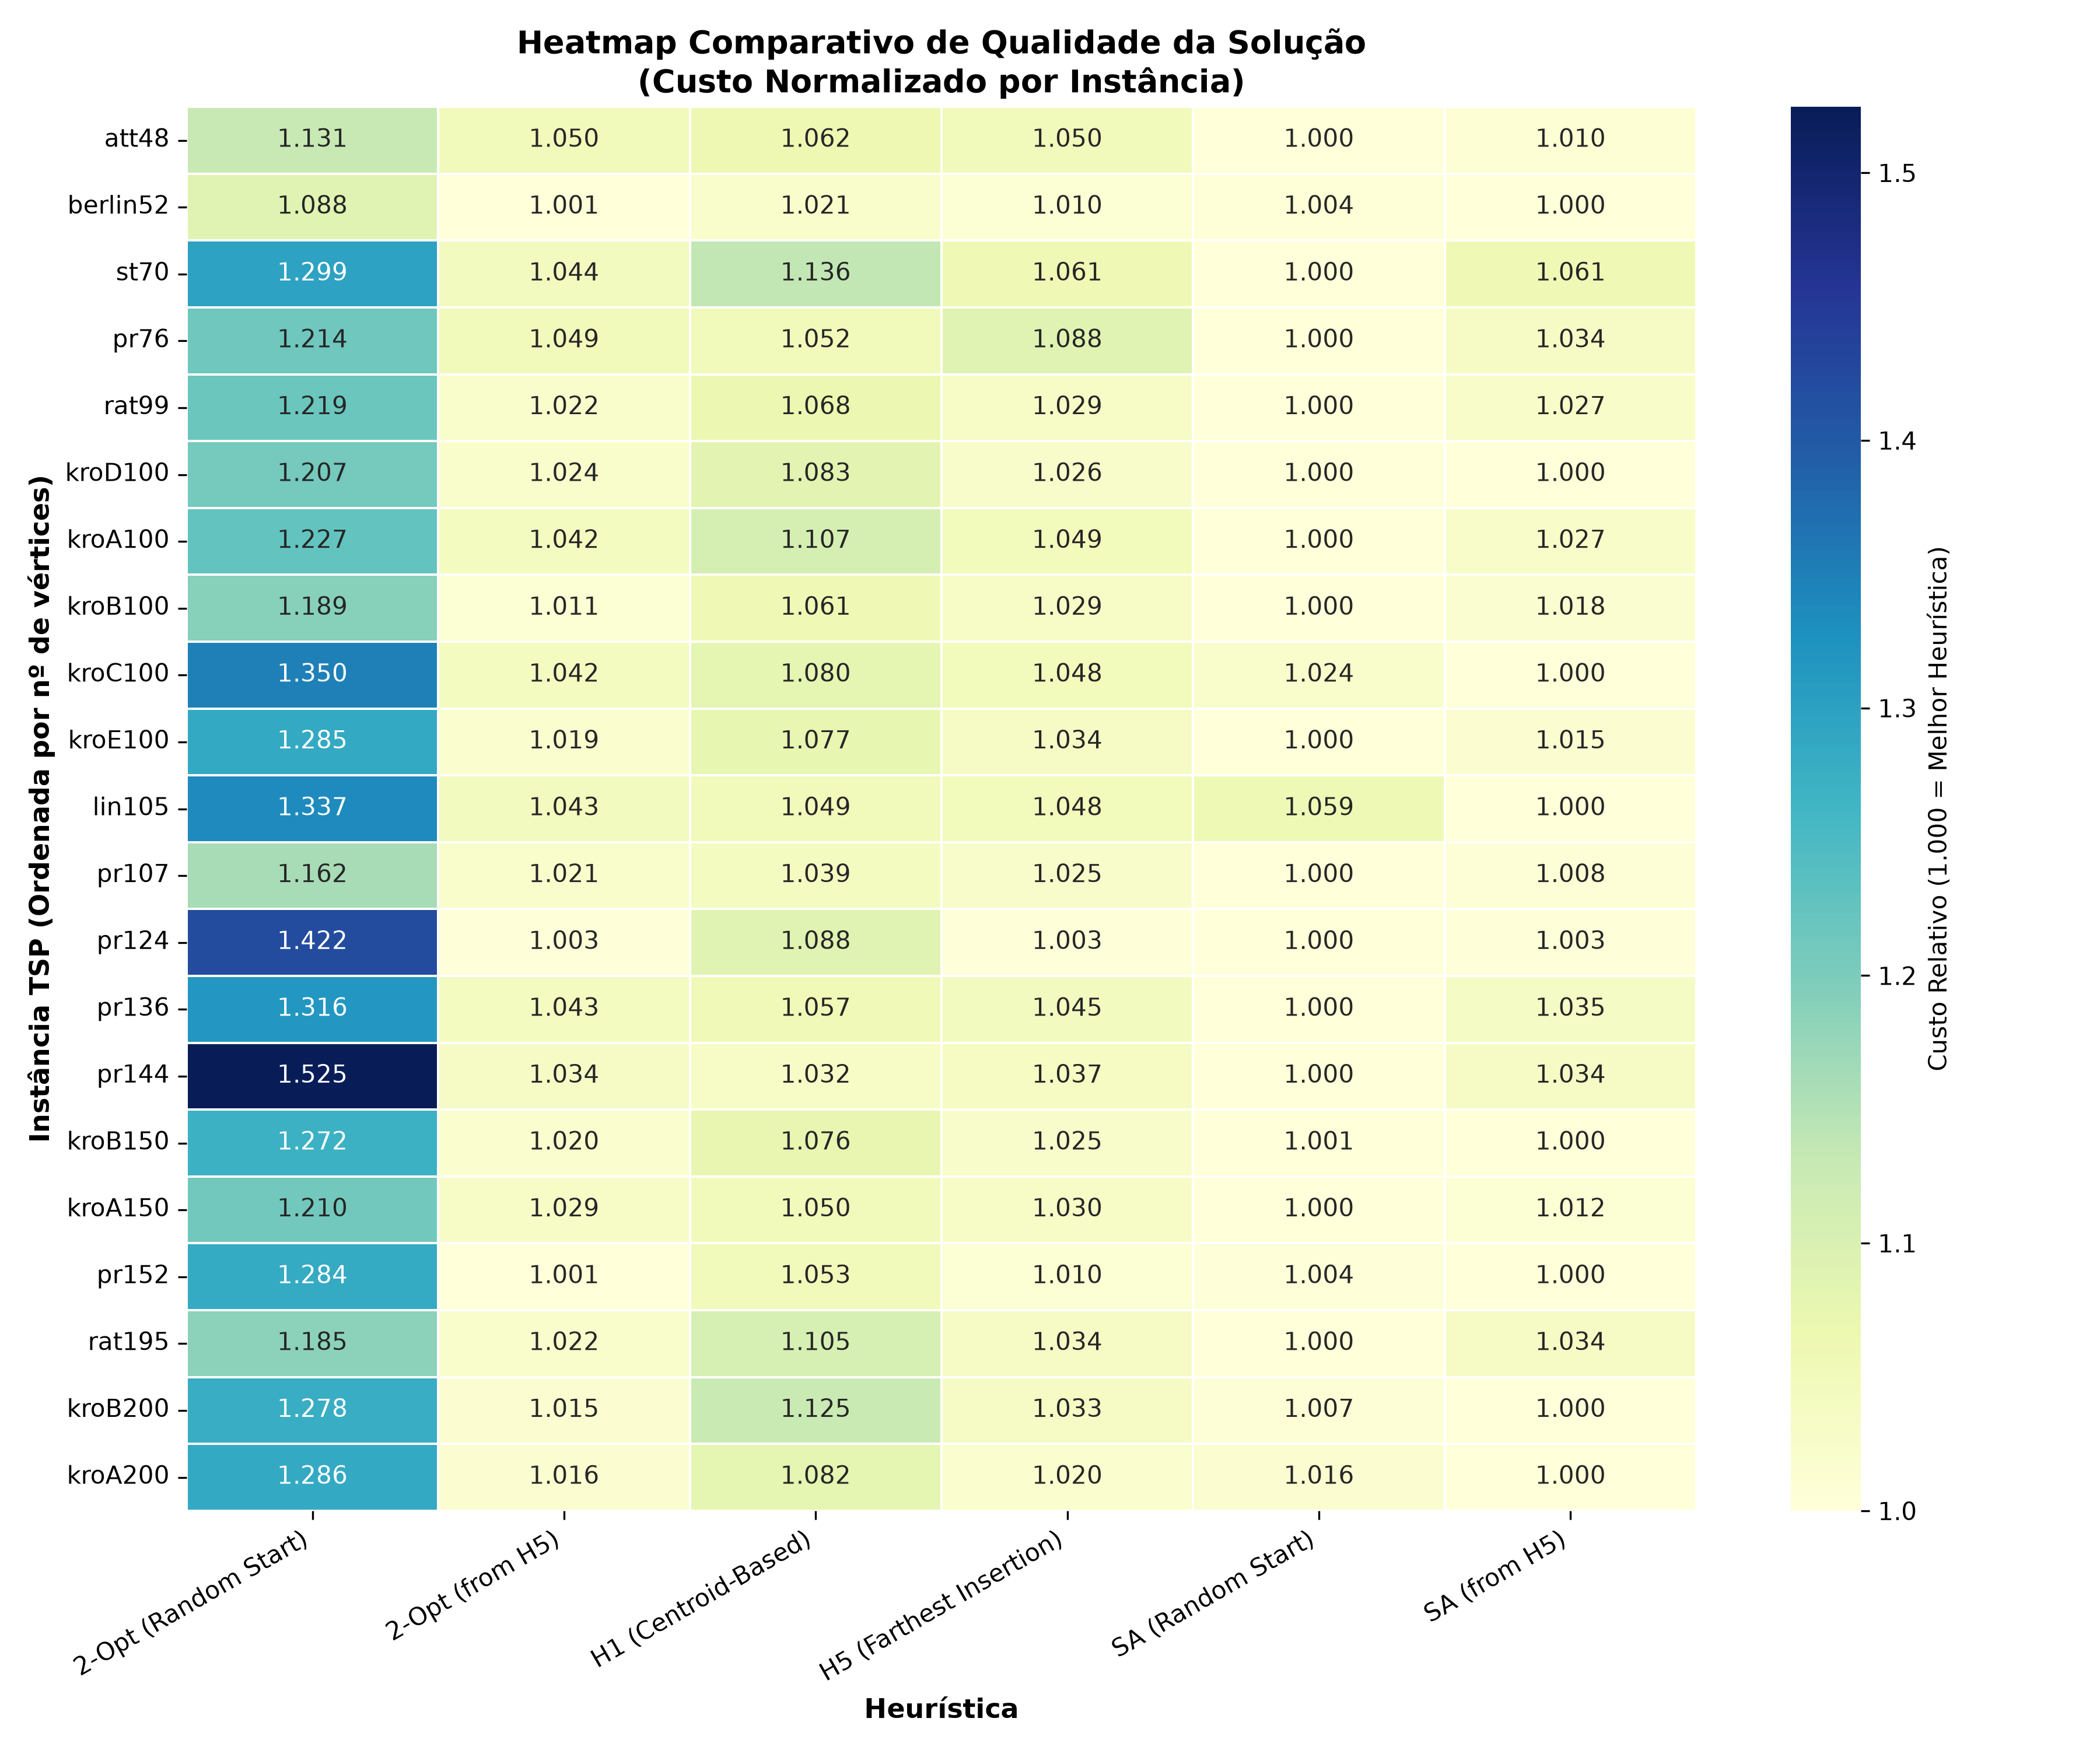
\includegraphics[width=0.95\textwidth]{heatmap_custo_relativo.png}
    \caption{\textit{Heatmap} do Custo Relativo por instância e método ($1{,}000$ = melhor solução).}
    \label{fig:heatmap_custo_meta}
\end{figure}

Observa-se que o SA (Random Start) e o SA (from H5) exibem coloração clara uniforme em toda a extensão da matriz. O 2-Opt (from H5) mostra-se consistentemente superior a H5 e H1. Em contrapartida, o 2-Opt (Random Start) apresenta coloração escura persistente, com perdas severas de qualidade que chegam a $1{,}524\times$ em \texttt{kroC100} e $1{,}477\times$ em \texttt{pr144}.

\subsection{\textit{Heatmap} de Tempo Computacional}

A Figura~\ref{fig:heatmap_tempo_meta} apresenta a distribuição do tempo computacional em milissegundos.

\begin{figure}[H]
    \centering
    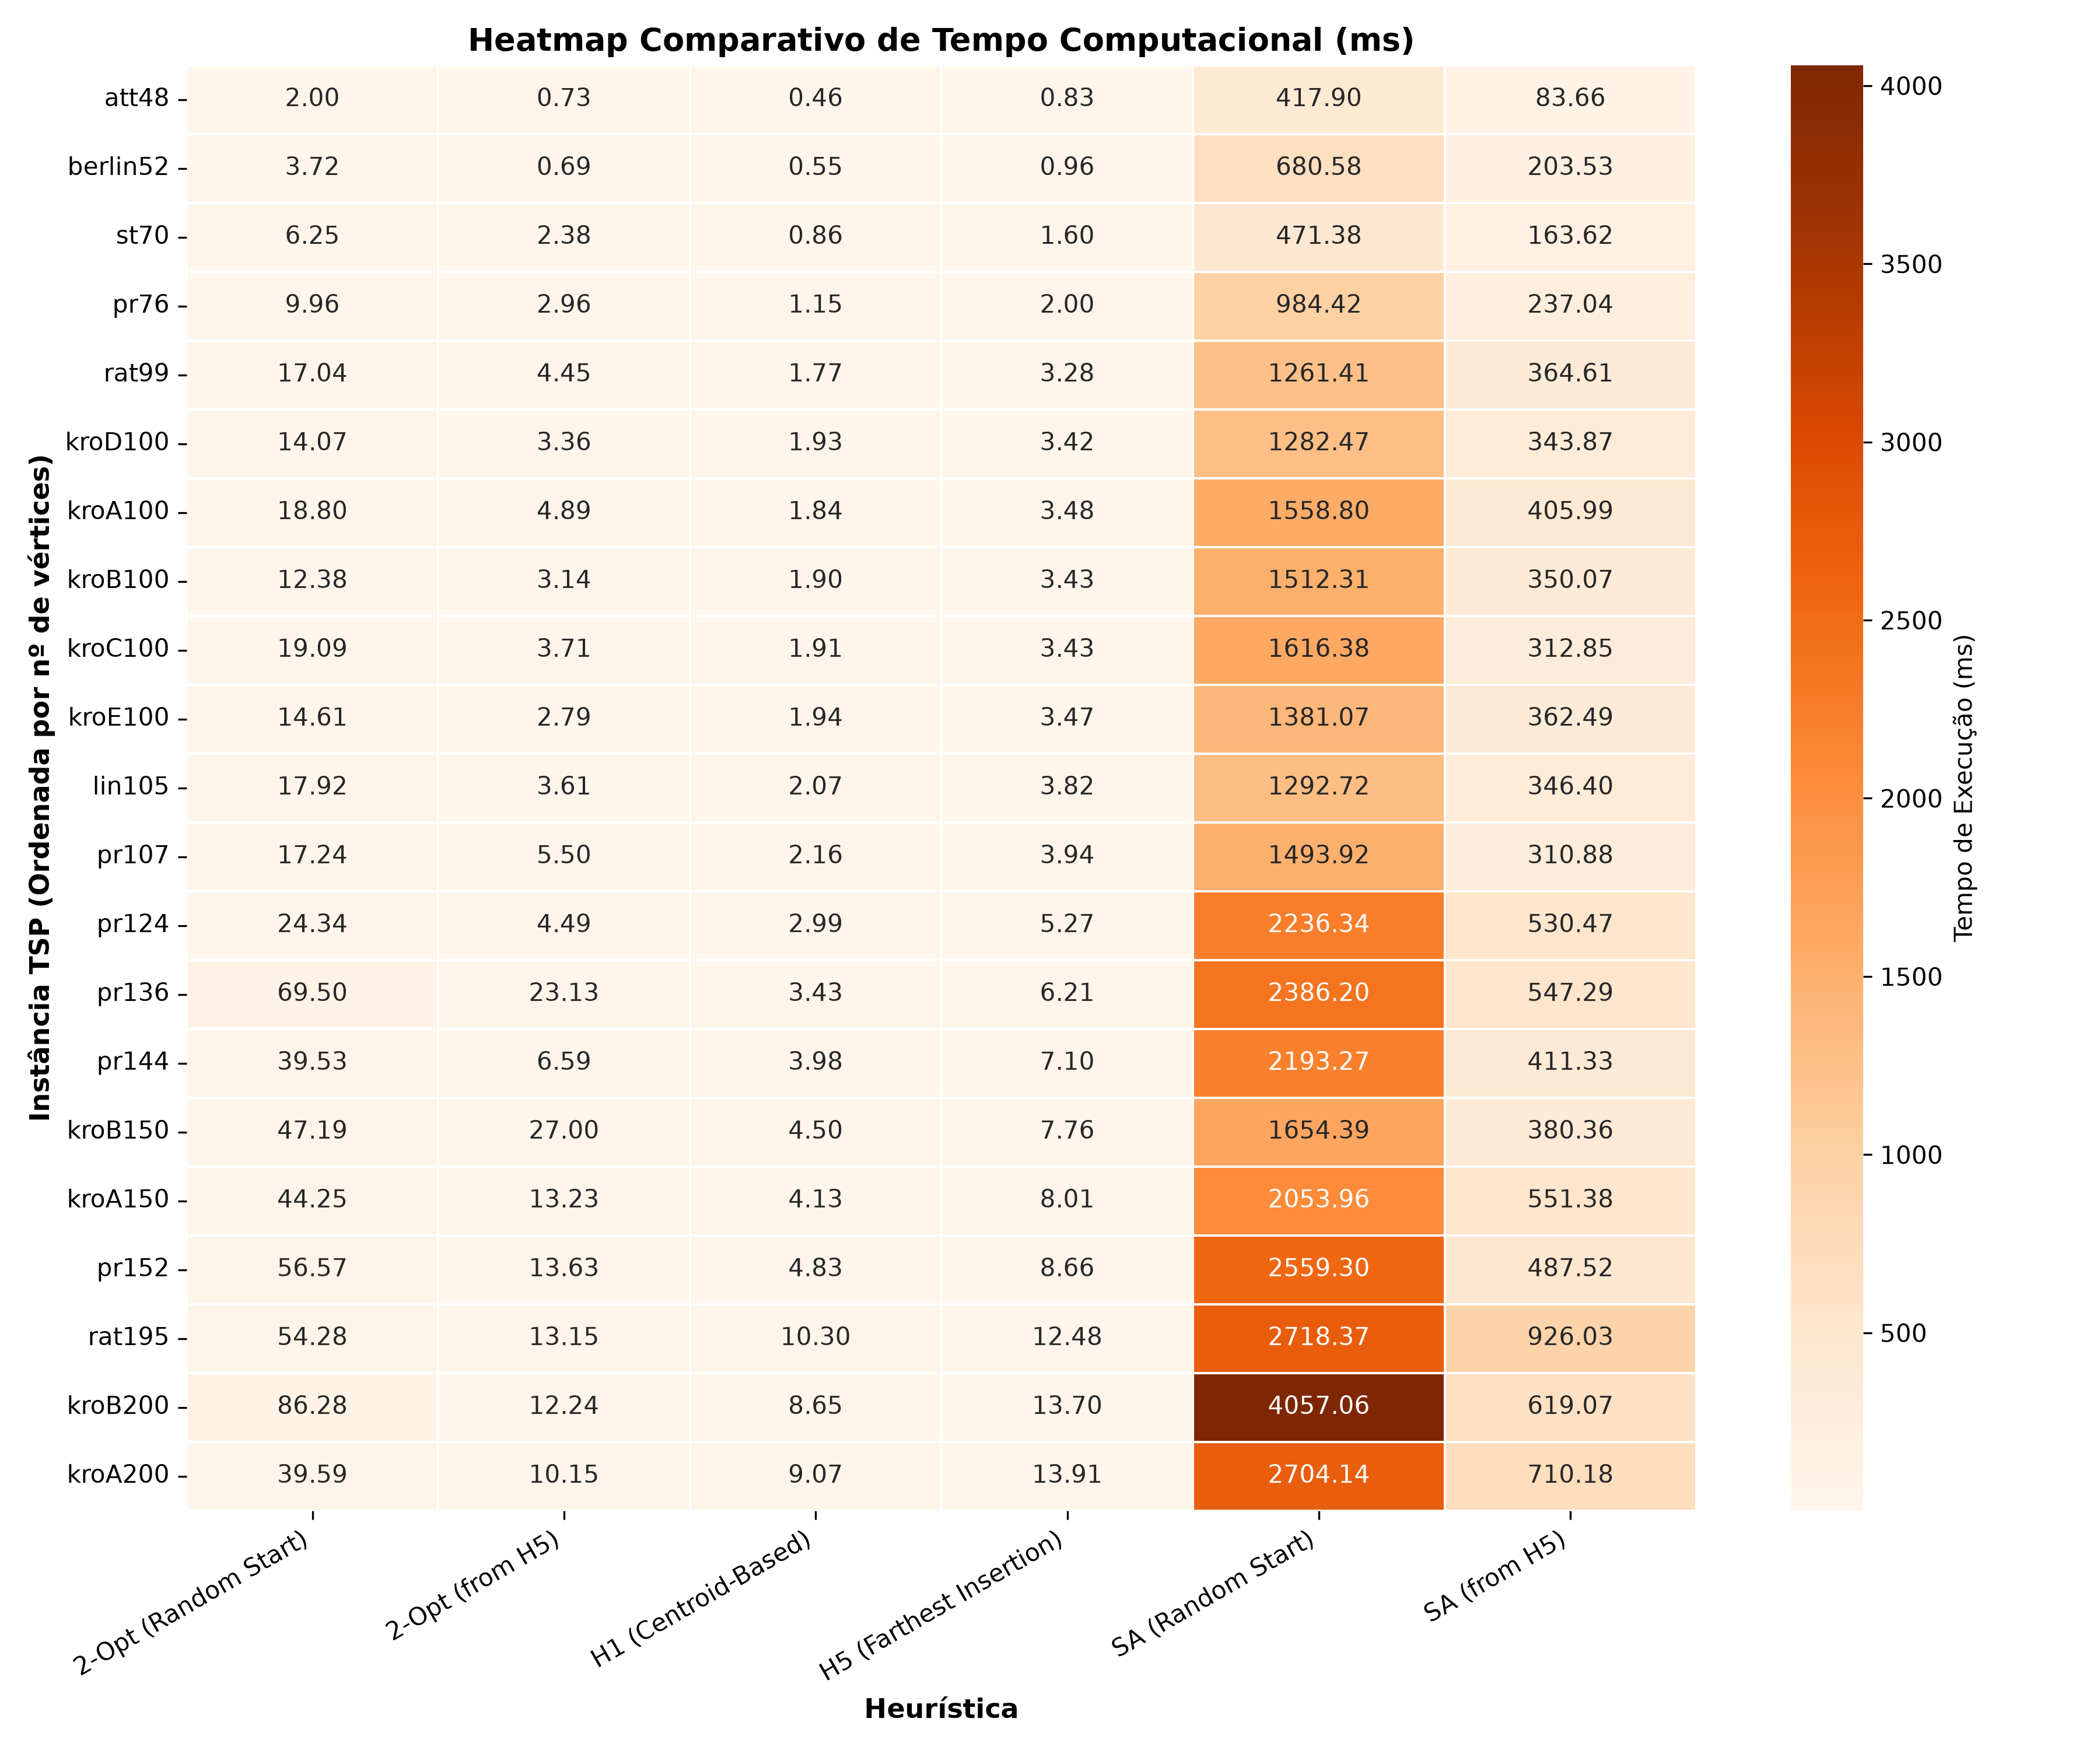
\includegraphics[width=0.95\textwidth]{heatmap_tempo_execucao.png}
    \caption{\textit{Heatmap} do tempo de execução em milissegundos por instância e abordagem.}
    \label{fig:heatmap_tempo_meta}
\end{figure}

Destacam-se três regimes operacionais: ultrabaixa latência (abaixo de $15\,\mathrm{ms}$), que inclui H1, H5 e 2-Opt (from H5); latência intermediária ($100$ a $900\,\mathrm{ms}$), ocupada pelo SA (from H5); e regime intensivo ($1$ a $4\,\mathrm{s}$), ocupado pelo SA (Random Start) nas instâncias com maior número de nós.

\subsection{\textit{Boxplot} de Custo Relativo}

A Figura~\ref{fig:boxplot_custo_meta} ilustra a dispersão estatística do Custo Relativo.

\begin{figure}[H]
    \centering
    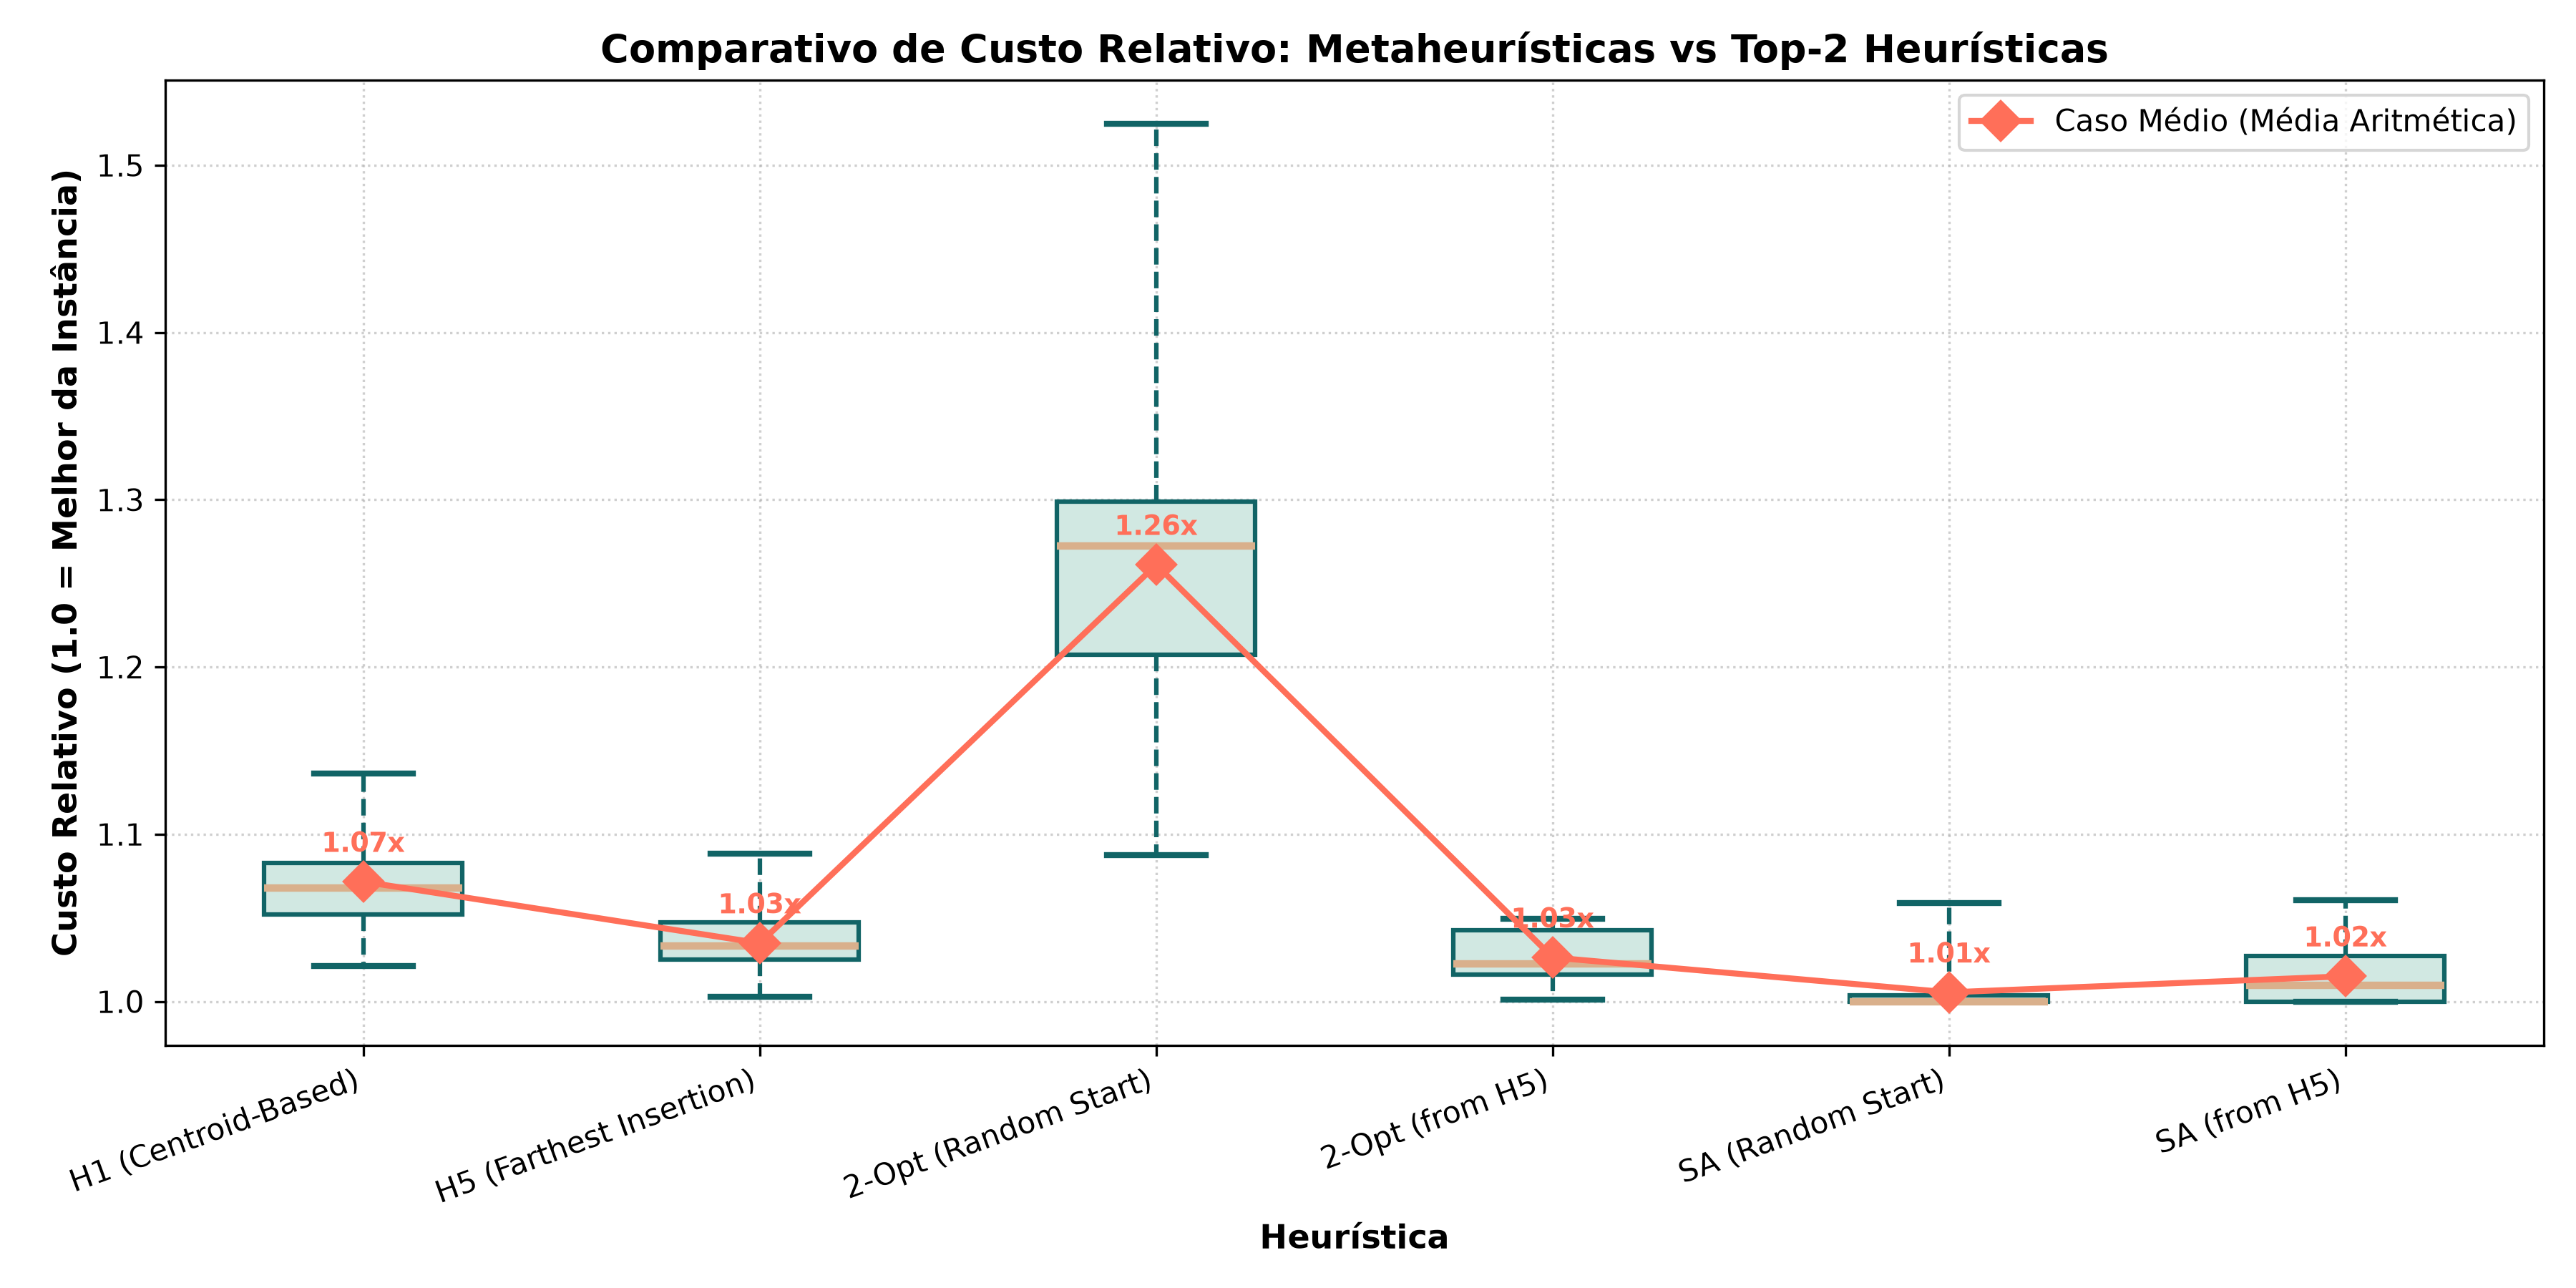
\includegraphics[width=0.95\textwidth]{boxplot_custo_relativo_metaheuristicas.png}
    \caption{Distribuição do Custo Relativo nas 21 instâncias (o diamante indica a média).}
    \label{fig:boxplot_custo_meta}
\end{figure}

Ambas as variantes de SA apresentam caixas interquartis muito estreitas com desvios mínimos. O 2-Opt (from H5) também demonstra estabilidade elevada (desvio-padrão de $0{,}0157$), enquanto o 2-Opt (Random Start) apresenta dispersão massiva com amplitude de $1{,}087$ a $1{,}525$.

\subsection{\textit{Boxplot} de Tempo de Execução}

A Figura~\ref{fig:boxplot_tempo_meta} ilustra a distribuição estatística do tempo de CPU consumido.

\begin{figure}[H]
    \centering
    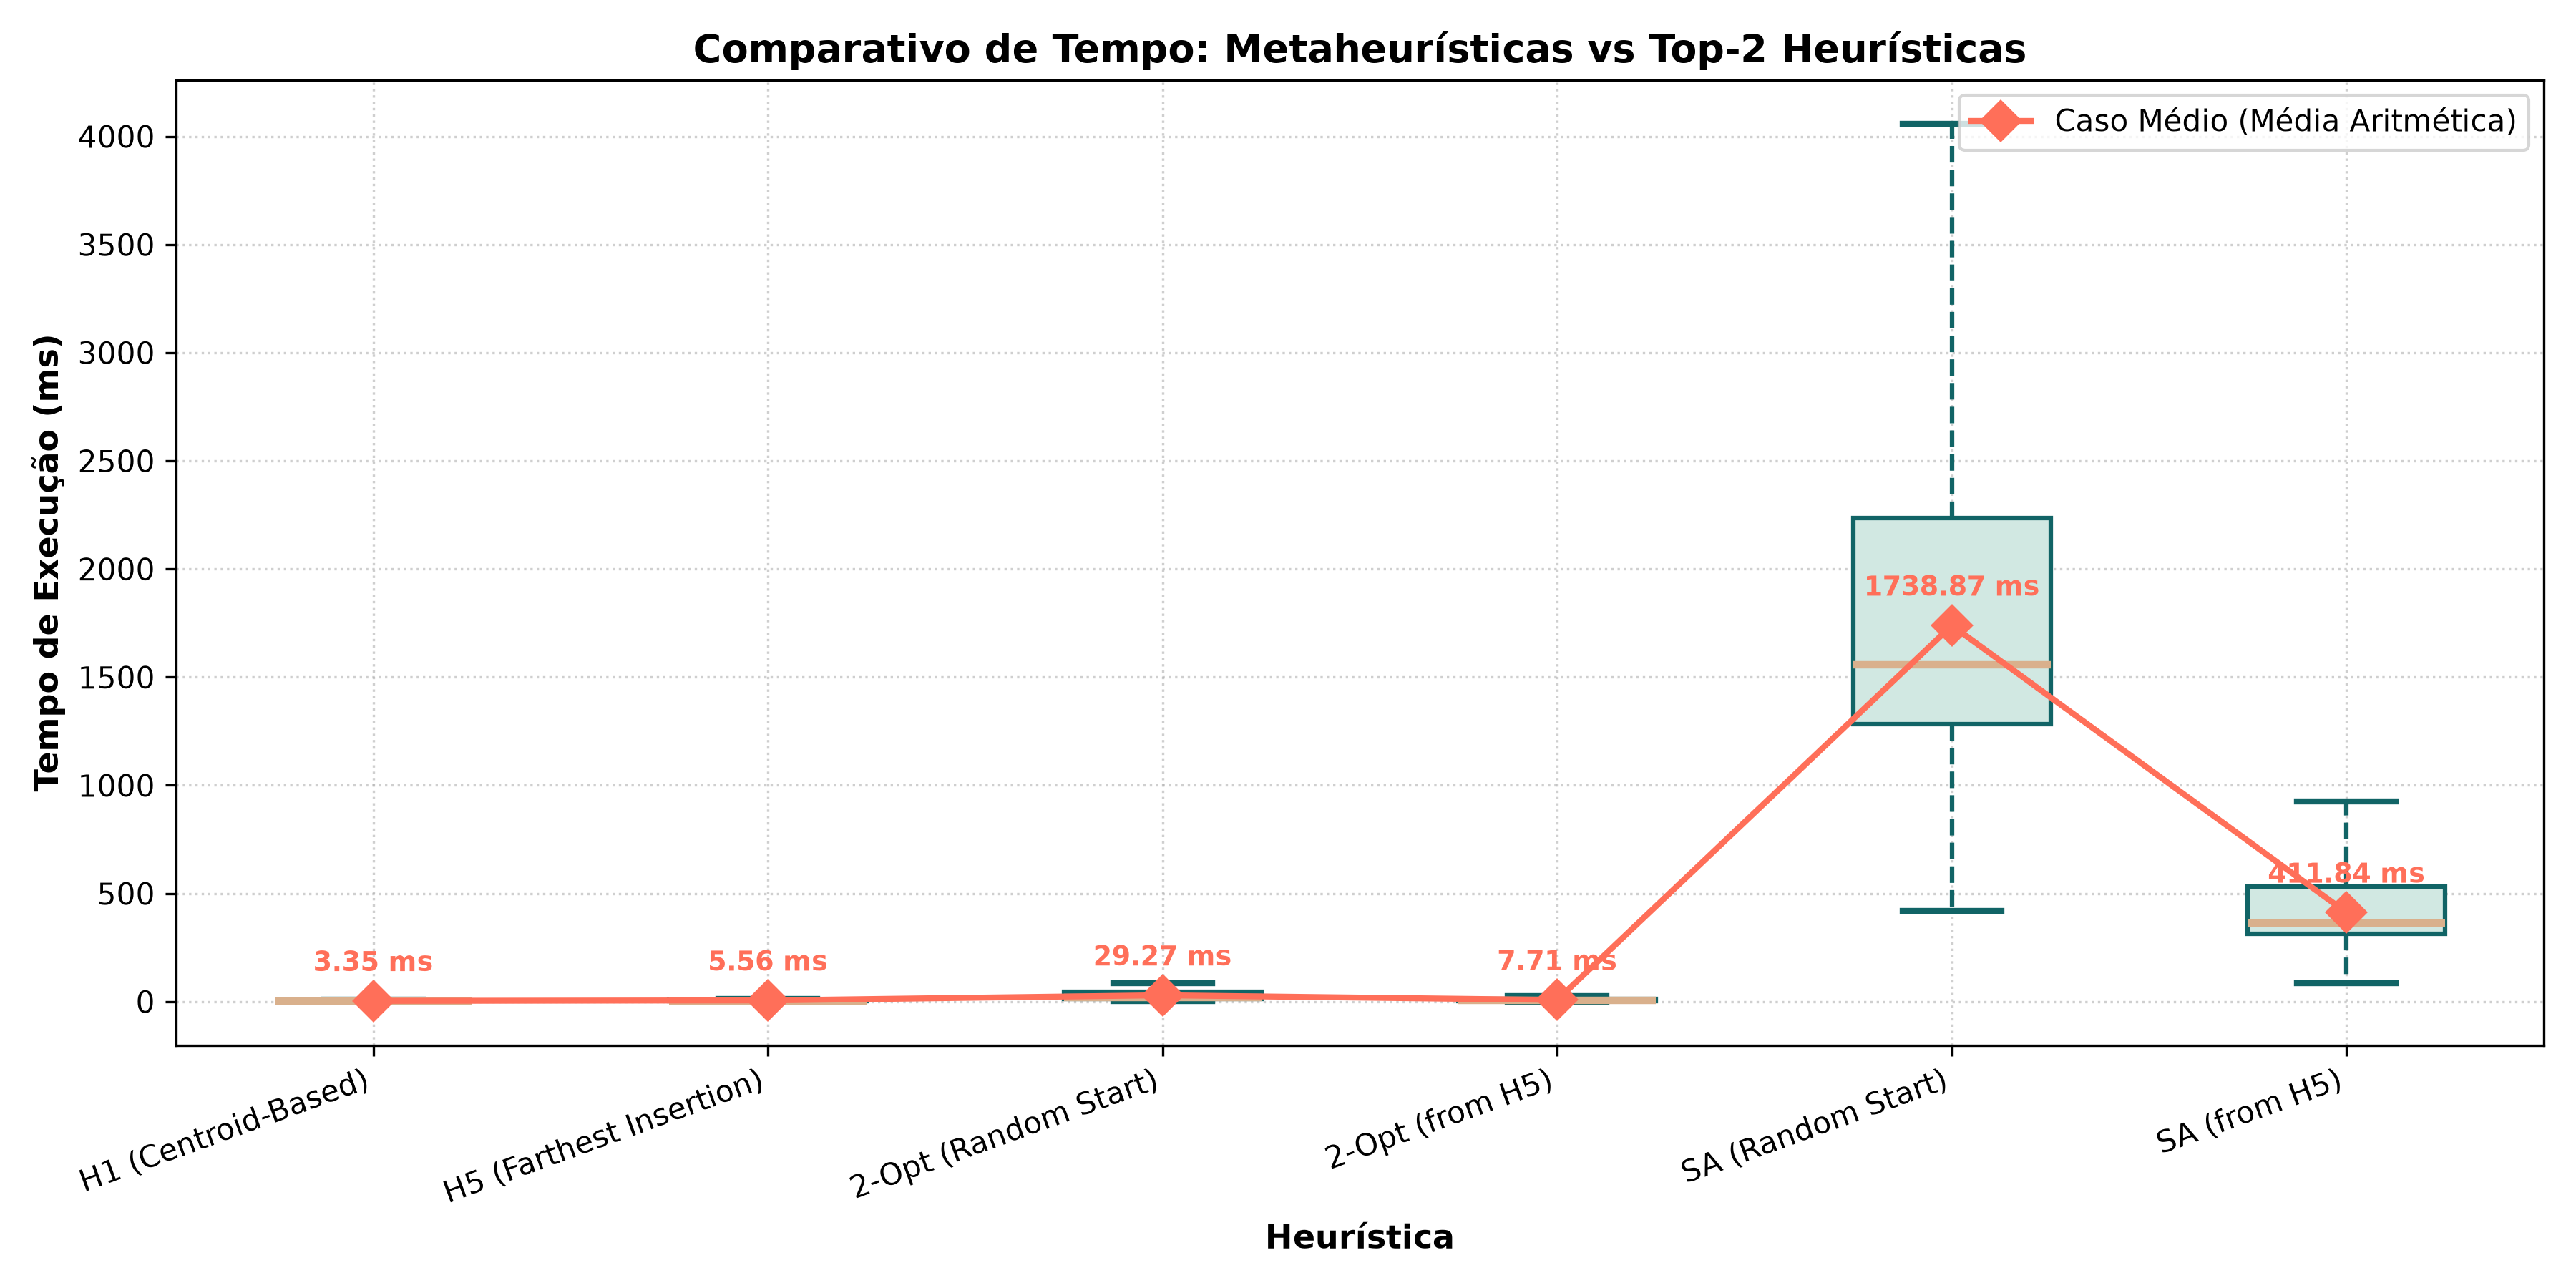
\includegraphics[width=0.95\textwidth]{boxplot_tempo_metaheuristicas.png}
    \caption{Distribuição do tempo de execução em milissegundos por método.}
    \label{fig:boxplot_tempo_meta}
\end{figure}

Verifica-se a grande estabilidade dos tempos das abordagens construtivas e do 2-Opt híbrido (mediana de $4{,}48\,\mathrm{ms}$ no 2-Opt from H5 vs $18{,}8\,\mathrm{ms}$ no 2-Opt randômico).

\subsection{Fronteira de Pareto Multiobjetivo}

A Figura~\ref{fig:pareto_meta} projeta as metodologias no espaço biobjetivo relacionando Custo Médio e Tempo Médio de Execução.

\begin{figure}[H]
    \centering
    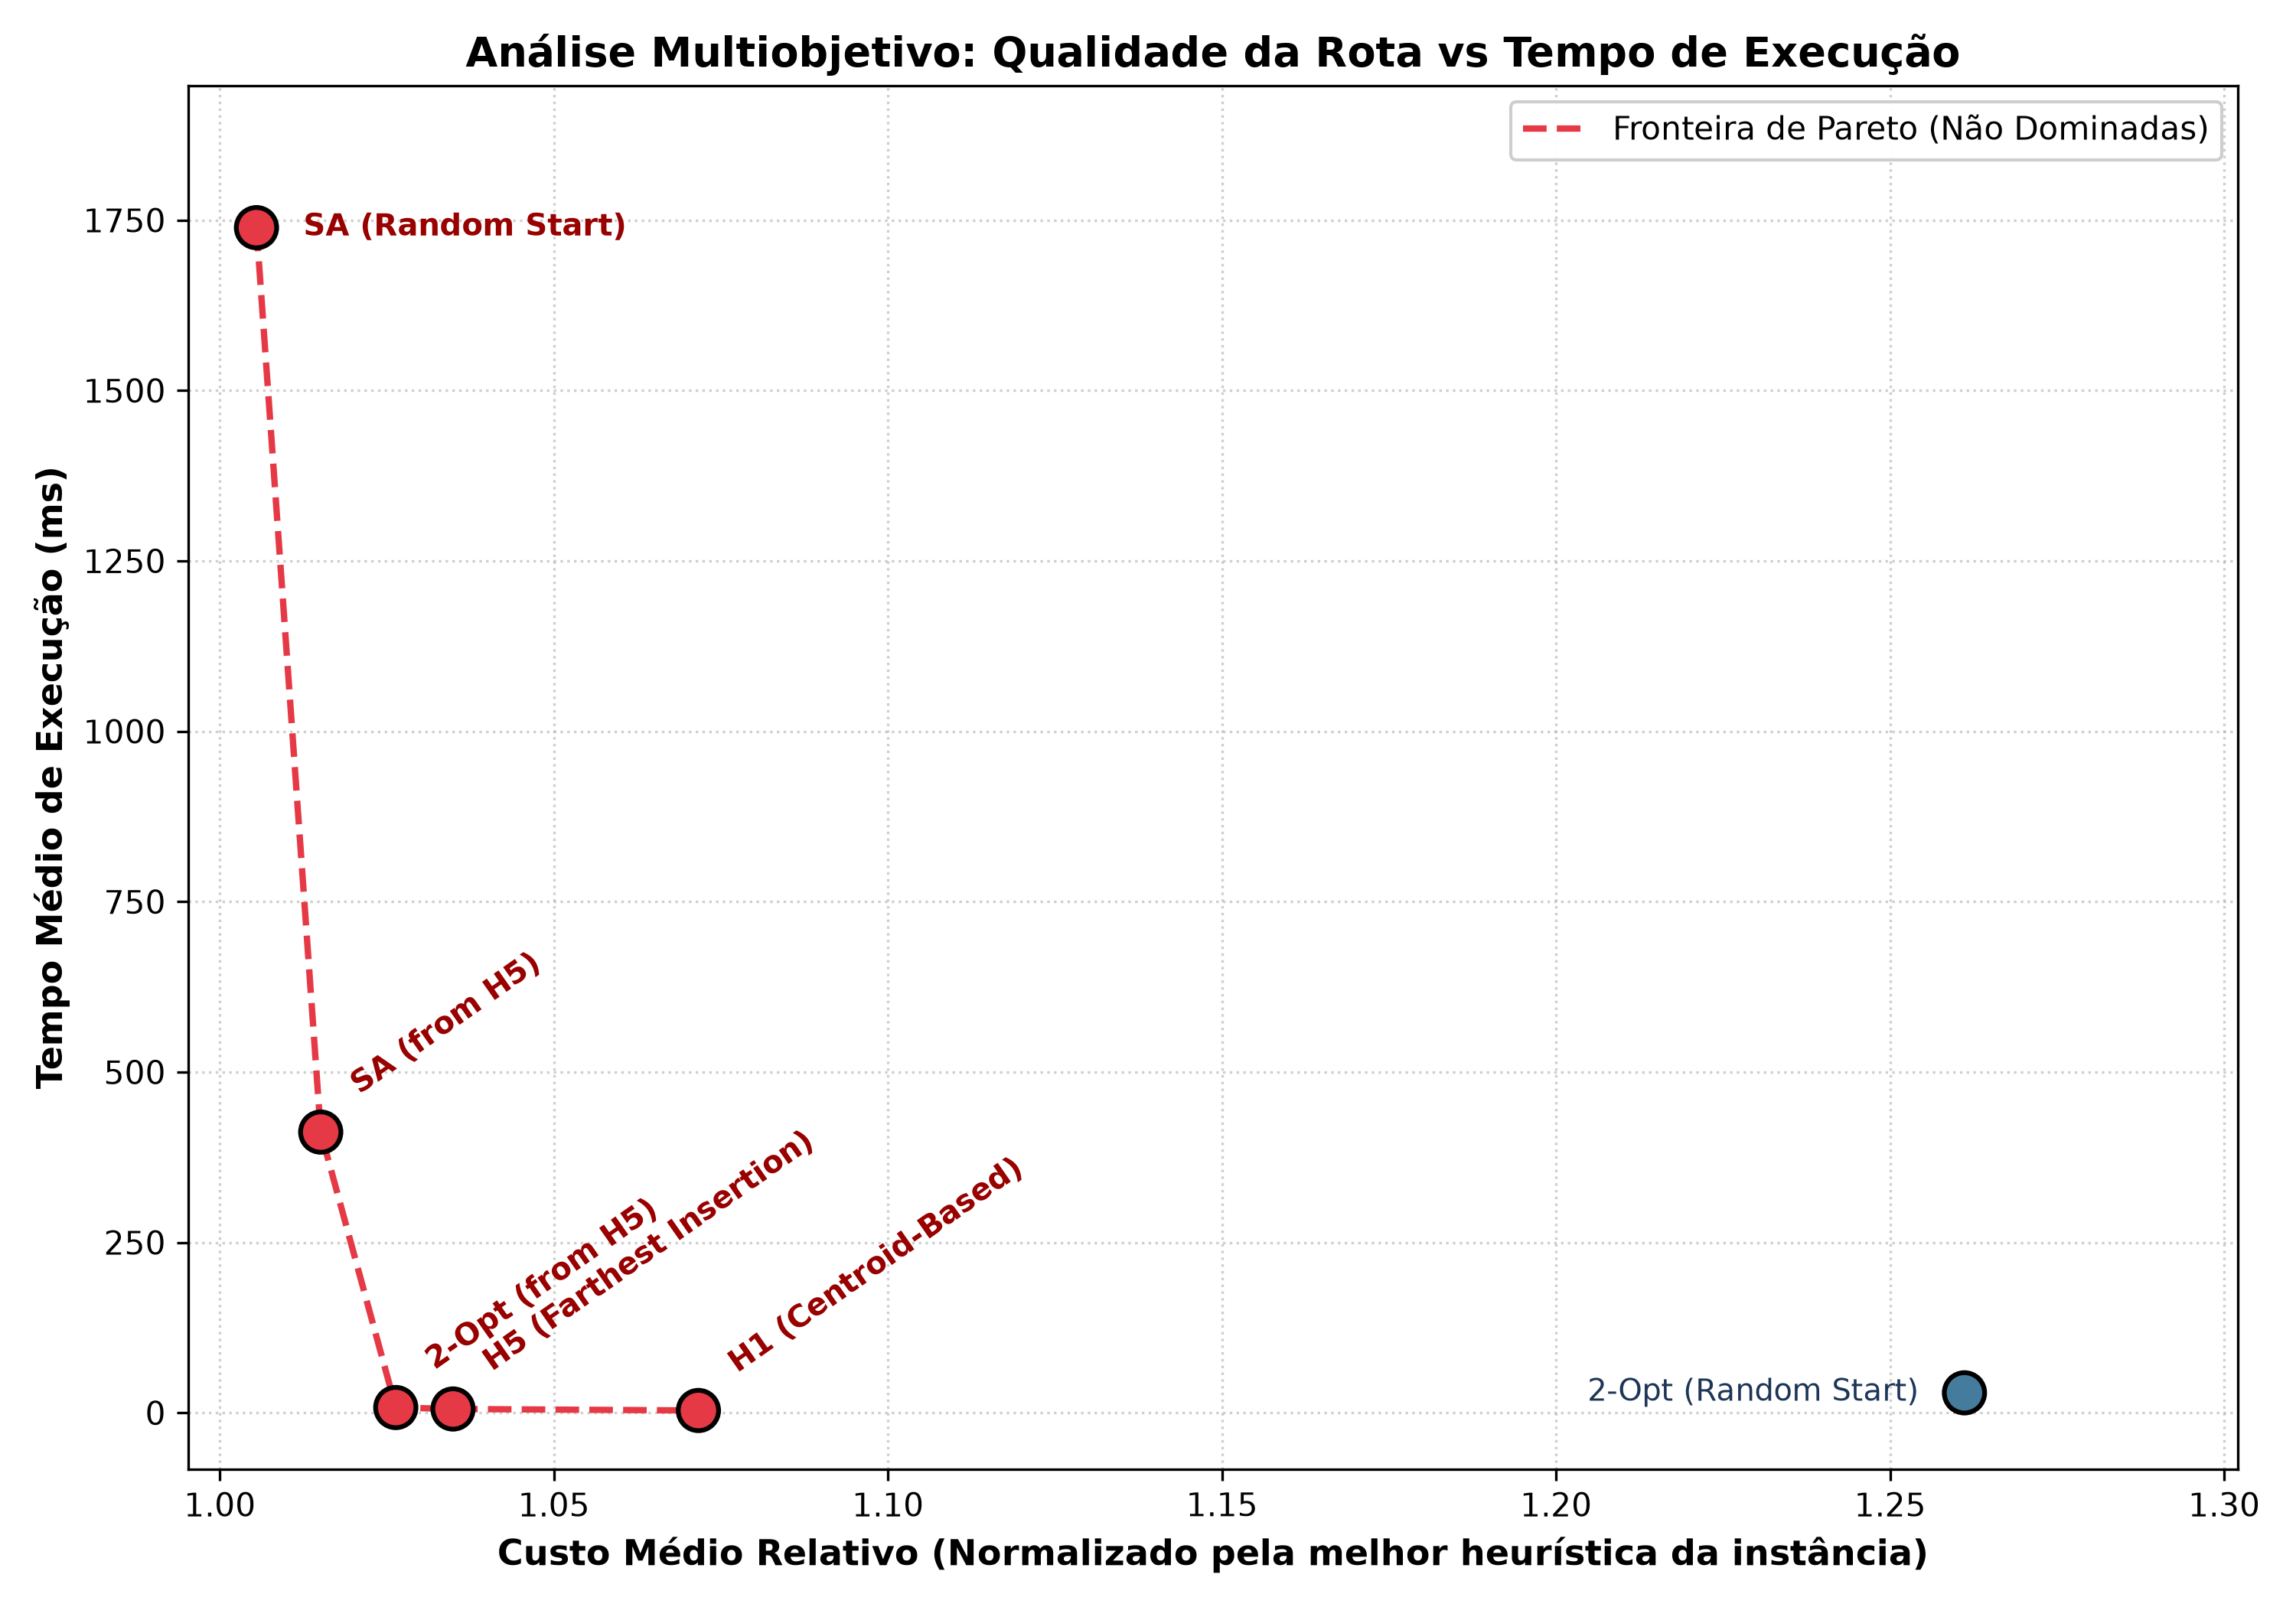
\includegraphics[width=0.95\textwidth]{pareto_metaheuristicas.png}
    \caption{Fronteira de Pareto relacionando Custo Médio e Tempo Médio de Execução.}
    \label{fig:pareto_meta}
\end{figure}

Os pontos não dominados que compõem a Fronteira de Pareto são:
\begin{enumerate}
    \item \textbf{H1 (\textit{Centroid-Based})}: extremo de menor latência ($3{,}35\,\mathrm{ms}$, custo $36.292$).
    \item \textbf{H5 (\textit{Farthest Insertion})}: ponto não dominado na faixa ultrarrápida ($5{,}56\,\mathrm{ms}$, custo $35.429$), apresentando qualidade superior a H1 com tempo inferior a qualquer variante de busca local ou metaheurística.
    \item \textbf{2-Opt (from H5)}: ponto de equilíbrio de eficiência operacional ($7{,}71\,\mathrm{ms}$, custo $35.067$), reduzindo o custo em relação ao H5 puro com acréscimo temporal de apenas $2{,}15\,\mathrm{ms}$.
    \item \textbf{SA (from H5)}: transição para regimes de alta acurácia ($411{,}84\,\mathrm{ms}$, custo $34.692$).
    \item \textbf{SA (Random Start)}: qualidade máxima global ($1.738{,}87\,\mathrm{ms}$, custo $34.247$).
\end{enumerate}
A única abordagem que se situa no interior dominado da fronteira é o \textbf{2-Opt (Random Start)}, sendo estritamente superada simultaneamente em custo e em tempo computacional por H1, H5 e 2-Opt (from H5).

% -------------------------------------------------------
\section{Discussão Comparativa Aprofundada}
% -------------------------------------------------------

\subsection{Comparativo entre as Metaheurísticas e Busca Local}

O confronto entre Busca Local 2-Opt e \textit{Simulated Annealing} evidencia a distinção teórica entre descida estrita e metaheurística global estocástica. Em permutações aleatórias, o 2-opt elimina cruzamentos triviais de forma desordenada, gerando amarrações topológicas que demandariam trocas de 3 ou mais arestas para serem desfeitas. Por aceitar apenas $\Delta < 0$, o algoritmo fica irreversivelmente bloqueado. Já o SA utiliza o critério de Metropolis para aceitar pioras temporárias na fase de alta temperatura, permitindo escapar dessas bacias de atração e reorganizar a rota antes da cristalização do circuito.

\subsection{Papel do Warm Start e Low-Temperature Start}

A comparação com as soluções de partida confirma os postulados de Johnson e McGeoch \cite{johnson1997}:
\begin{itemize}
    \item \textit{Warm Start no 2-Opt}: a rota inicial de H5 já estabelece a conformação macroscópica correta; o 2-Opt atua apenas removendo torções locais residuais deixadas pelas últimas inserções, reduzindo o custo de $35.429$ para $35.067$ em apenas $7{,}71\,\mathrm{ms}$.
    \item \textit{Low-Temperature Start no SA}: inicializar o SA em temperatura reduzida a partir de H5 evita a destruição estocástica da macroestrutura, convergindo em $411\,\mathrm{ms}$ (mais de 4 vezes mais rápido que a partida aleatória) com acurácia a $1{,}5\%$ da melhor solução global.
\end{itemize}

% -------------------------------------------------------
\section{Conclusões}
% -------------------------------------------------------

A avaliação experimental desenvolvida neste trabalho permitiu analisar o comportamento, a convergência e o custo computacional de duas técnicas avançadas de otimização no TSP --- a Busca Local 2-Opt acelerada por \textit{Don't-Look Bits} e o \textit{Simulated Annealing} (SA) --- sob estratégias de partida aleatória e partida informada via \textit{warm start}.

Os resultados experimentais conduzem às seguintes conclusões centrais sobre as metaheurísticas avaliadas:

\begin{enumerate}
    \item \textbf{Limitações da Busca Local 2-Opt Isolada}: A execução da busca local 2-opt a partir de permutações aleatórias revelou-se ineficaz, apresentando o pior desempenho médio do benchmark ($1{,}2611\times$, correspondente a cerca de $26\%$ acima do melhor custo) e tempo elevado ($29{,}27\,\mathrm{ms}$) decorrente do esforço excessivo para eliminar nós desestruturados. Em contraste, quando empregado como operador de pós-otimização sobre uma rota previamente estruturada (\textit{Warm Start}), o 2-Opt demonstra alta eficácia, corrigindo cruzamentos residuais em apenas $7{,}71\,\mathrm{ms}$ e atingindo custo relativo médio de $1{,}0263\times$.

    \item \textbf{Eficácia Global do Simulated Annealing (SA)}: A capacidade estocástica de transpor barreiras energéticas através do critério de Metropolis garantiu ao SA a maior acurácia de todo o estudo. Sob inicialização aleatória e resfriamento térmico amplo, a metaheurística obteve a melhor solução em 14 das 21 instâncias da TSPLIB ($1{,}0055\times$ de custo relativo médio), demandando em média $1{,}74\,\mathrm{s}$ de processamento.

    \item \textbf{Vantagem do Low-Temperature Start no SA}: A inicialização em baixa temperatura a partir de uma rota pré-estruturada provou ser altamente vantajosa para o SA, reduzindo o tempo de convergência em mais de $76\%$ ($411{,}84\,\mathrm{ms}$ contra $1.738{,}87\,\mathrm{ms}$) com perda residual mínima de qualidade ($1{,}0151\times$, sendo a melhor solução em 7 instâncias). Essa parametrização preserva as sub-rotas benéficas descobertas na rota base e concentra o esforço computacional no refinamento estocástico fino.

    \item \textbf{Trade-off entre Busca Local e Metaheurística Estocástica}: A seleção entre Busca Local 2-Opt e \textit{Simulated Annealing} estabelece um compromisso nítido entre latência e precisão de rota. Para aplicações com restrições temporais severas na faixa de milissegundos, o 2-Opt refinado sobre \textit{warm start} constitui a alternativa mais eficiente, entregando soluções altamente competitivas com custo temporal insignificante. Para problemas em que a qualidade do circuito é prioritária e orçamentos computacionais de frações de segundo a poucos segundos são toleráveis, o \textit{Simulated Annealing} consolida-se como a metaheurística soberana.
\end{enumerate}

% -------------------------------------------------------
% Referências Bibliográficas
% -------------------------------------------------------
\bibliographystyle{plain}
\bibliography{referencias}

\end{document}
